\graphicspath{{./assets/}}
\setcounter{mtc}{1}
\chapter{Generalized context of the project }
\fancyhead[R]{\ungaramond\small\textbf{Chapter I. Generalized context of the project}}
\minitoc
\newpage
\section*{Introduction}


\section{Overview on the host organization  }
\section{Project description}
\section{Analysis of existing processes }

\section{Constructive criticism on existing processes }


\fancyhead[R]{\ungaramond\small\textbf{Chaptre 1: Generalized context of the project}}

\newpage

\section{Problem statement }
\section{Ideation and proposed solution  }
\section{Project management }
\subsection{Comparative research }


\begin{table}[h!]
\center
\begin{tabular}[b]{|m{3cm}|m{4cm}|m{4cm}|m{4cm}|}
\hline
\rowcolor{white}
 & Waterfall (V model) 
 & Agile   & DevOPS  \\
\hline
 Lifecycle  
& Linear software development approach 
& Incremental and iterative sprint cycles. 
& Uses automation techniques to enable continuous deployment of change. \\
\hline
 Automation level  
& Low 
& Varied 
& High 
 \\
\hline
 Delivery of value 
& Slow (Scale : months) 
& Rapid (daily/weekly) 
& Continuous  \\
\hline
 Responsiveness to business needs 
& Extremely limited 
& Responsive 
& Highly responsive   \\
\hline
 Collaboration 
& Low: teams operate in functional silos 
& Improved: short dev cycles 
& High: cross-functional teams are involved from project start. \\
\hline
Quality 
& Low: issues are only identified after tests 
& Improved: issues are identified after every sprint 
& High: Unit testing and code quality checks are performed during development. \\
\hline
 Risk 
& Increases as project development progresses 
& Decreases as project development progresses 
& Decreases as project development progresses \\
\hline
\end{tabular}
\caption{Table comparatif research}
\textcolor{white}{I} \label{tab:tab-m}
\end{table}

Based on the previous comparative study, it is apparent that the approach most suited to our use case is one that helps improve collaboration, reduce context-switching, introduce automation, and enable observability and monitoring. 

\subsection{Agile devSecOPS }

When evaluating devSecOPS as a practice and Agile as a delivery approach, it is important to note that they are not mutually exclusive. In spite of the evident differences between DevSecOPS and the Agile methodology, their overall goal of increasing speed and delivering quality software is similar in nature and together they produce great products and improve the software development. 

The following figure showcases an overview of the process and the key DevSecOPS roles. 

\begin{figure}[!ht]\centering
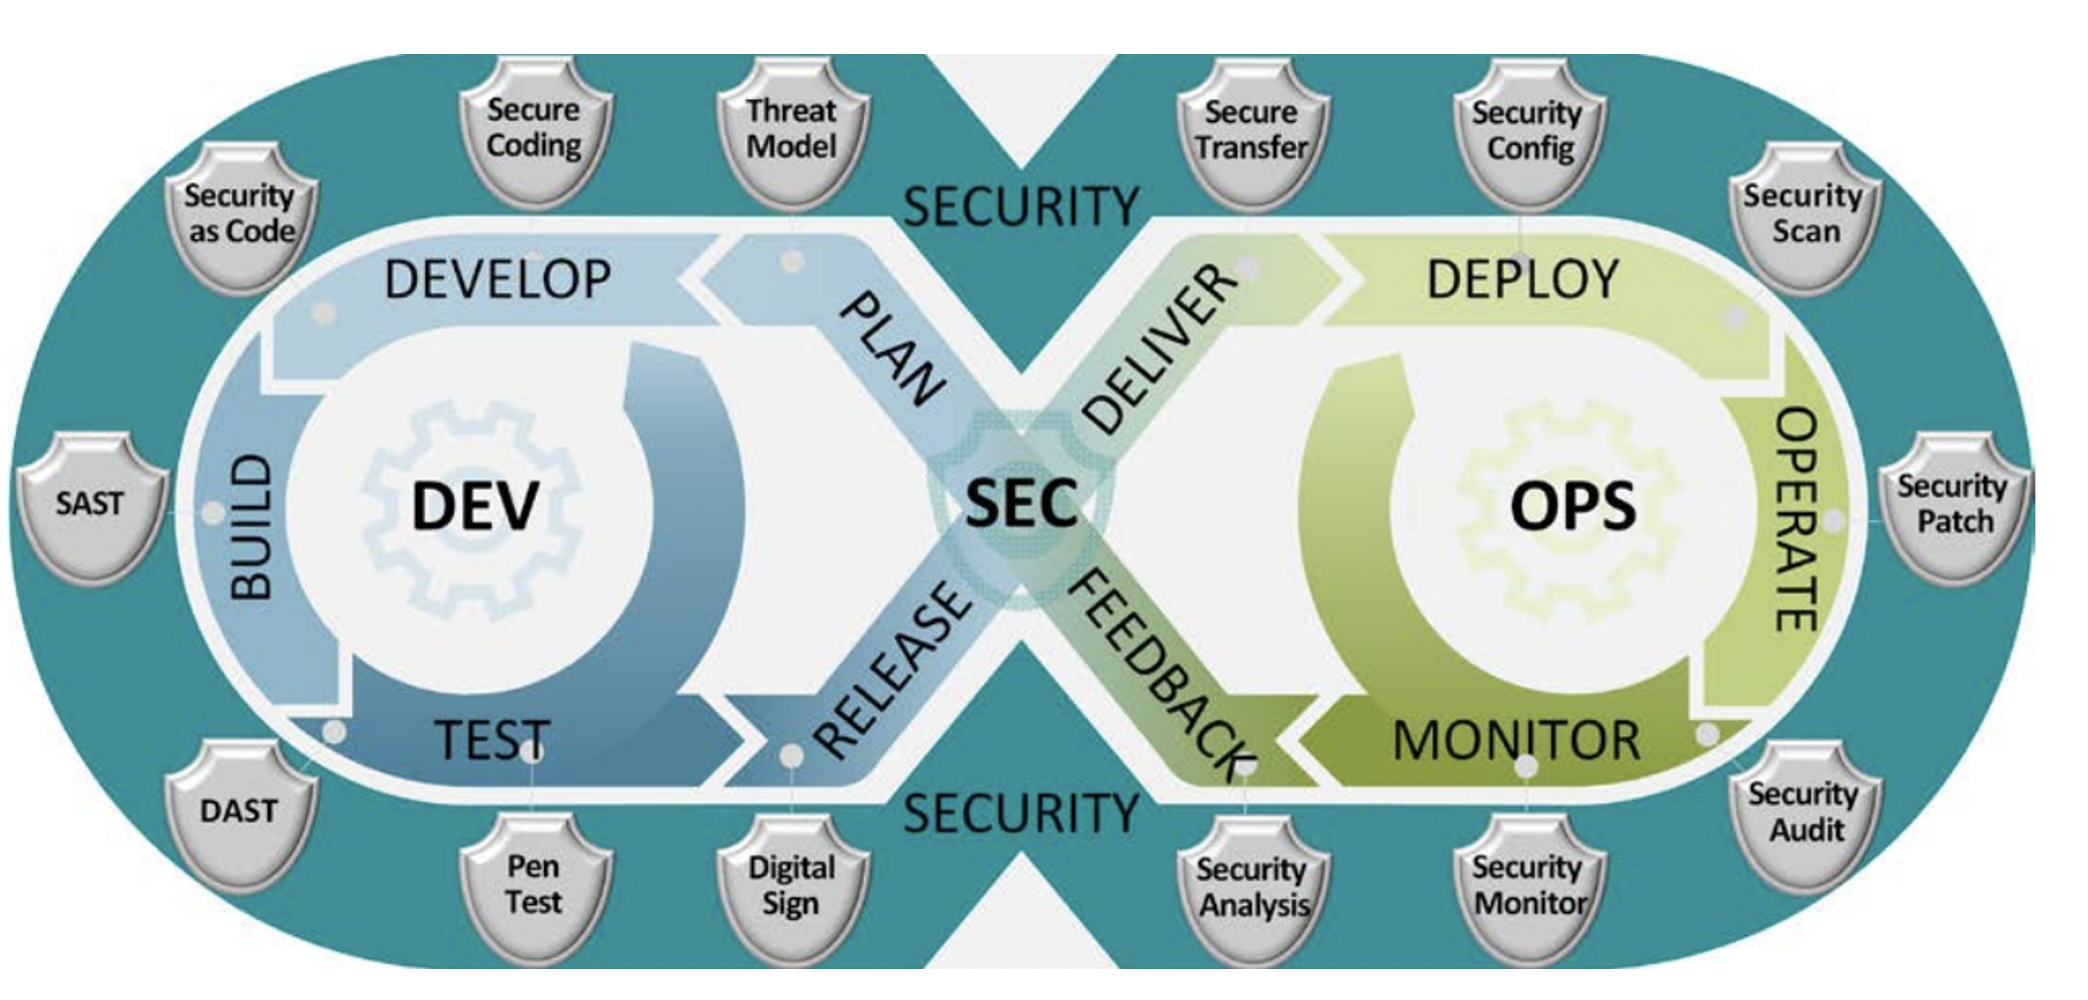
\includegraphics[width=0.8\textwidth,angle=00]{assets/f1.png}
\caption{Process overview}
\label{fig:processOverview}
\end{figure}


\paragraph{DevSecOPS Evangelist:} 
Usually the DevSecOPS team leader, he focuses on promoting the DevSecOPS advantages, identifying and quantifying companies’ benefits deriving from a higher agility. 

\paragraph{Release Manager:} 
The product stability manager which is basically the product owner. He cares about the product’s management and coordination. 

\paragraph{Automation Architect: }
Provides a complete automation role involving the DevSecOPS and Cloud solutions. He is an integration specialist that ensures the high availability of the pre-production and production systems. 

\paragraph{Software Developer/Tester:}
DevSecOPS developers are not responsible only for the transformation of new requirements into code, they also have to deal with testing, distribution and continuous monitoring processes.

\paragraph{Security Engineer: }
The DevSecOPS approach implements security by design.


